%%%%%%%%%%%%%%%%%%%%%%%%%%%%%%%%%%%%%%%%%%%%%%%%%%%%%%%%%%%%%%%%%%%%%%
%%%%%%%%%%%%%%%%%%%%%%%%%%%%%%%%%%%%%%%%%%%%%%%%%%%%%%%%%%%%%%%%%%%%%%
%%
%% IVT LaTeX template
%%   Kevin Riehl
%%   kevin.riehl@ivt.baug.ethz.ch
%%   
%%   Updates
%%   01.07.2019 | First version of overleaf compatible template for IVT. (Dr. Joseph Molloy)
%%   15.12.2019 | Add german abstract page and fix bug in figure indenting. (Dr. Joseph Molloy)
%%   15.02.2025 | New LaTeX Revision to solve compilation issues & simplify.
%%
%%%%%%%%%%%%%%%%%%%%%%%%%%%%%%%%%%%%%%%%%%%%%%%%%%%%%%%%%%%%%%%%%%%%%%
%%%%%%%%%%%%%%%%%%%%%%%%%%%%%%%%%%%%%%%%%%%%%%%%%%%%%%%%%%%%%%%%%%%%%%
%% This is an example for writing a paper at the IVT.
%% It supports English and German language.
%% Include german option in document class for german headings (i.e. Literatur)
%% \documentclass[numbered, german]{ivt-style/standard}
%%%%%%%%%%%%%%%%%%%%%%%%%%%%%%%%%%%%%%%%%%%%%%%%%%%%%%%%%%%%%%%%%%%%%%
%%%%%%%%%%%%%%%%%%%%%%%%%%%%%%%%%%%%%%%%%%%%%%%%%%%%%%%%%%%%%%%%%%%%%%
\documentclass[numbered]{ivt-style/standard}

\newcommand{\mlc}[1]{}

\usepackage{amsmath}
\usepackage{amsthm}
\usepackage{amsfonts}
\usepackage{amssymb}
\usepackage{listings}
\usepackage{minted}
\usepackage{float}
\usepackage{placeins}
\usepackage{hyperref}

\RequirePackage[capitalize]{cleveref}
\RequirePackage{booktabs}
\RequirePackage{natbib}
\providecommand{\ivthline}{}

\title{Reservoir Computing: Implementation and Analysis}
\subtitle{Study Oriented Project}
\papertype{Final Report}
\headingstitle{Reservoir Computing}

\author{
  \textcolor{red}{Vimarsh Shah} \\
  Department of Physics \\
  BITS Pilani \\
  Goa \\
  \texttt{\textcolor{red}{f20221060@goa.bits-pilani.ac.in}}
  % \and
  % Second Author \\
  % IVT \\
  % ETH Zurich
  % \and
  % Third Author \\
  % IVT \\
  % ETH Zurich
  % \and
  % Fourth Author \\
  % IVT \\
  % ETH Zurich
}

\reportdate{April 2025}
% \reportdategerman{April 2025}
\reportnumber{10XX}
% \titlefigure{figures/title_RC}

\titlefigure{ivt-style/rc_intro_matplotlib}
%%%% If you don't want to include an english abstract page, comment out this command
\abstract{
Reservoir computing (RC) offers an alternative paradigm for analysing time series derived from dynamical systems. Utilising a fixed, randomly connected internal network (the reservoir), RC requires training only a linear output layer, thereby reducing the computational complexity associated with conventional recurrent neural network training. This report provides an overview of RC fundamentals, covering the echo state property necessary for processing temporal information, a comparison with standard recurrent networks, and a summary of its principal advantages and limitations. 

The report also details implementations and applications of RC principles, specifically using an Extreme Learning Machine (ELM) as the time-series predictor, to analyse data from the logistic map. The input data consists of noisy time series generated at various parameter settings, designed to emulate data acquired from physical systems like electronic circuits subject to inherent noise. Principal Component Analysis (PCA) is applied to the output weights derived from training the ELM on these datasets, facilitating the estimation of the underlying parameter space (the bifurcation locus). Subsequently, the trained ELM is employed to generate the reconstructed bifurcation diagram across this estimated parameter range. We compare this architecture with other ones using different non-linear systems as well as Recurrent Neural Networks (RNNs). The results are presented, evaluating the capability of this RC-based approach to approximate the true system dynamics and its performance when dealing with the noise present in the input data.


The complete code with different tests and experiments conducted is available on \href{https://github.com/vimarsh244/ResorvoirComputing_SOP}{GitHub}.

 }
%%% To inclue a second abstract page with german headings and a german abstract, use the command below
% \germanabstract{
%     Dieser Bericht....
% }
% \keywords{keyword1, keyword2, etc}
% \suggestedCitation{Fill in the suggested citation format for your paper here}

\begin{document}
\maketitle
\clearpage

\tableofcontents

% \listoffigures

\newpage

%%%%%%%%%%%%%%%%%%%%%%%%%%%%%%%%%%%%%%%%%%%%%%%%%%%%%%%%%%%%%%%%%%%%%%
%% Main Text
%%%%%%%%%%%%%%%%%%%%%%%%%%%%%%%%%%%%%%%%%%%%%%%%%%%%%%%%%%%%%%%%%%%%%%


\section{Introduction}

Machine learning has transformed numerous fields through its ability to extract patterns from data and make predictions without explicit programming. Traditional deep learning approaches often rely on gradient-based optimisation of neural network weights through backpropagation. While effective for many applications, these methods face challenges when dealing with recurrent neural networks (RNNs) designed to process sequential or temporal data.

RNNs are theoretically well-suited for temporal tasks due to their cyclical connections that enable information persistence across time steps. However, training RNNs presents significant difficulties, particularly the vanishing or exploding gradient problem during backpropagation through time as well the time taken to train a Neural Network. This challenge has motivated researchers to explore alternative approaches to harnessing the power of recurrent architectures.

Reservoir computing emerges in this context as a solution that maintains the representational power of recurrent networks while dramatically simplifying the training process. By leveraging a fixed, randomly initialised recurrent network (the reservoir) and only training the output connections, RC offers a computationally efficient approach to temporal modelling with several distinct advantages:

\begin{itemize}
    \item Simplified training through linear regression of output weights only
    \item Reduced computational demands compared to full RNN training
    \item Ability to process temporal information through the reservoir's inherent memory
    \item Adaptability to physical implementations in various substrates
\end{itemize}

\begin{figure}[H]
    \centering
    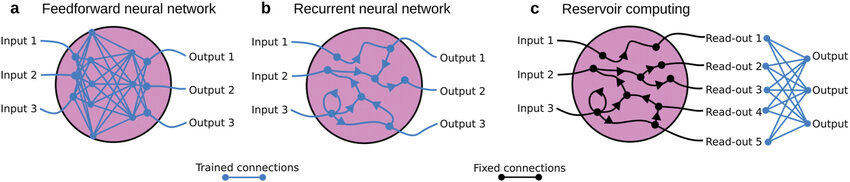
\includegraphics[width=1.0\linewidth]{figures/rc_difference_with others.png}
    \caption{Illustration of (a) a feedforward neural network (FNN) with its acyclic and trainable connections, (b) a recurrent neural network featuring trainable feedback and cyclic connections, and (c) a reservoir made of untrained connections. For RC, only the connection between readout layer and output layer is trained, typically with a linear regression.}
    \label{fig:rc_diff}
    \cite{article_RC_intro}
\end{figure}

This report explores the fundamentals of reservoir computing, examines implementation strategies, and analyzes results from reproducing experiments described in recent literature. 


\section{Basics of Reservoir Computing}

\subsection{General Principle}
Reservoir computing is a computational framework that transforms input signals into output signals through a high-dimensional, nonlinear dynamical system (the reservoir). The key distinction from traditional neural networks is that the reservoir's internal connections remain fixed and random, while only the readout layer is trained. \cite{article_RC_intro}


The general workflow of reservoir computing consists of three main components:
\begin{itemize}
    \item \textbf{Input Layer:} Maps external inputs to the reservoir through fixed, randomly initialised connection weights
    \item \textbf{Reservoir:} A recurrent network with random, fixed internal connections that creates a high-dimensional representation of the input
    \item \textbf{Output Layer:} A linear readout mechanism trained to map the reservoir states to desired outputs
\end{itemize}    

When an input signal enters the system, it triggers complex dynamics within the reservoir, creating a high-dimensional nonlinear transformation of the original input. This transformation preserves temporal information from past inputs through the reservoir's recurrent connections. The output layer then extracts relevant features from this rich representation through a simple linear combination of reservoir states.

A typical discrete-time reservoir update can be written as 
\[
\mathbf{x}[n+1] = f\bigl(\mathbf{W}\mathbf{x}[n] + \mathbf{W}^{\mathrm{in}}\mathbf{u}[n] + \mathbf{b}\bigr),
\]
where $\mathbf{x}[n]\in \mathbb{R}^N$ is the reservoir state at time step $n$, $\mathbf{u}[n]$ is the input vector, $\mathbf{W}$ is the (fixed, random) reservoir weight matrix, $\mathbf{W}^{\mathrm{in}}$ couples the input, and $f(\cdot)$ is a nonlinear activation (like $sigmoid$ or $\tanh$).  The reservoir may also include a bias $\mathbf{b}$.  The output of the network is then formed as a linear combination of the reservoir states and possibly the inputs:
\[
\mathbf{y}[n] = \mathbf{W}^{\mathrm{out}}\bigl[\mathbf{x}[n];\,\mathbf{u}[n]\bigr],
\]
where $\mathbf{W}^{\mathrm{out}}$ is the output weight matrix to be trained.  Only $\mathbf{W}^{\mathrm{out}}$ is adjusted during training, typically by solving a linear regression (often ridge regression) to fit target output sequences.  This greatly simplifies learning: by keeping $\mathbf{W}$ and $\mathbf{W}^{\mathrm{in}}$ fixed and random, training reduces to a linear algebra problem.  \cite{article_RC_intro} note that this means “one can use a random, untrained reservoir where only the output layer is optimised, for example, with linear regression”.  As a result, RC is extremely efficient to train compared to fully trainable recurrent networks, while still retaining rich nonlinear processing power.


While classical reservoirs are implemented in software simulations, an exciting trend is \emph{physical reservoir computing}.  Here, the reservoir is a physical system with inherent dynamics.  For example, optical, mechanical, or spintronic devices with nonlinear responses and short-term memory can serve as reservoirs. \cite{article_RC_intro} emphasises that many material systems “show nonlinear behaviour and short-term memory that may be harnessed to design novel computational paradigms”.  Using a physical reservoir can drastically speed up computation and circumvent some implementation issues of digital neural networks.  
We will later discuss a specific example: using a single physical oscillator (a pendulum) as a reservoir \cite{Mandal2022}. 

\subsection{Echo State Property and Fading Memory}

A critical property of effective reservoirs is the Echo State Property (ESP), which ensures that the reservoir's state depends only on a history of inputs and not on its initial conditions. In practical terms, this means that any influence of the initial reservoir state eventually fades away, allowing the system to respond consistently to the same input sequence regardless of starting conditions.

This property creates what is known as \textit{fading memory} - the reservoir retains information about recent inputs, with diminishing influence as inputs recede further into the past. This characteristic is essential for processing temporal information effectively.

Typically, this is achieved by scaling the spectral radius of $\mathbf{W}$ to be less than unity.  In practice, a reservoir should have enough \emph{memory capacity} to remember past inputs over a useful time horizon, but also enough nonlinearity to project inputs into a diverse feature space.  The memory capacity quantifies how many past time steps the reservoir state effectively retains.  A larger reservoir (more neurons or nodes) generally increases capacity, but too much memory can harm generalisation \cite{article_RC_intro}.  Nonlinearity (like the $\tanh$ activation or other nonlinear dynamics) is crucial as well, because it allows the reservoir to create complex combinations of inputs; the output layer then linearly combines these to approximate arbitrary functions of the inputs.


\subsection{Comparison with traditional RNNs}

Unlike traditional RNNs where all connection weights are optimised through backpropagation, reservoir computing leaves the recurrent connections fixed, typically with random values. This approach circumvents the vanishing/exploding gradient problem and significantly reduces computational complexity.

The comparison can be summarised as follows:

\paragraph{Traditional RNNs: }All connections (input, recurrent, and output) are trained through backpropagation through time, which is computationally intensive and may suffer from convergence issues.

\paragraph{Reservoir Computing:} Only output connections are trained, typically through simple linear regression (ridge regression), while input and recurrent connections remain fixed.

\subsection{Some Varients}

Two primary implementations of reservoir computing have been developed:

\paragraph{Echo State Networks (ESNs):} Introduced by \cite{article_esn_intro}, ESNs typically use rate-based neurons with continuous activation functions like tanh, with sparse random connectivity between reservoir units. 

\begin{figure}[H]
    \centering
    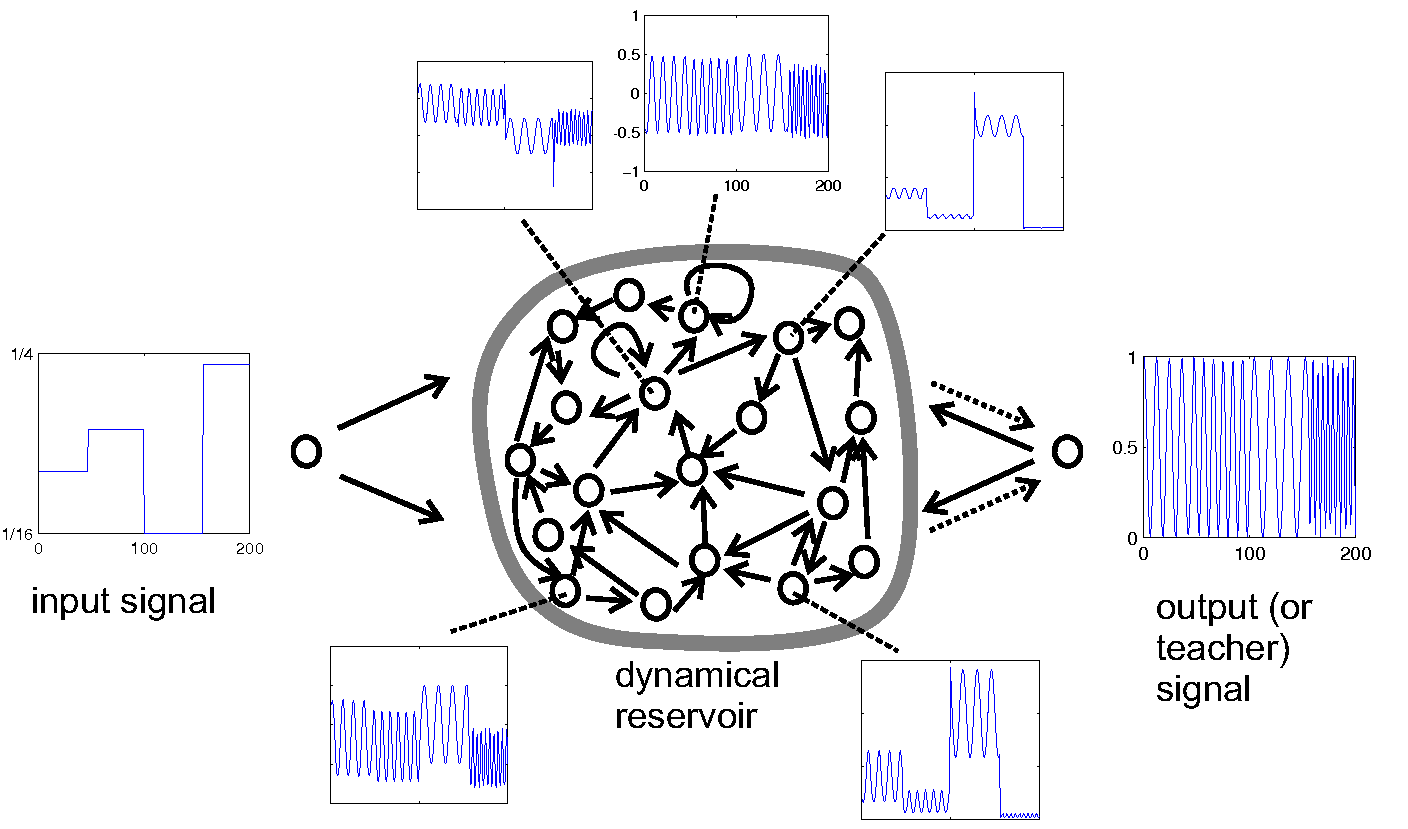
\includegraphics[width=1\linewidth]{figures/ESN_diag_FreqGenSchema.png}
    \caption{Echo State Network diagram. \cite{wiki:esn}}
    \label{fig:esn-diag}
\end{figure}
    
\paragraph{Liquid State Machines (LSMs):} Developed by \cite{article_lsm_intro}, LSMs use spiking neuron models that more closely resemble biological neurons. They were initially conceived in the context of computational neuroscience.

\begin{figure}[H]
    \centering
    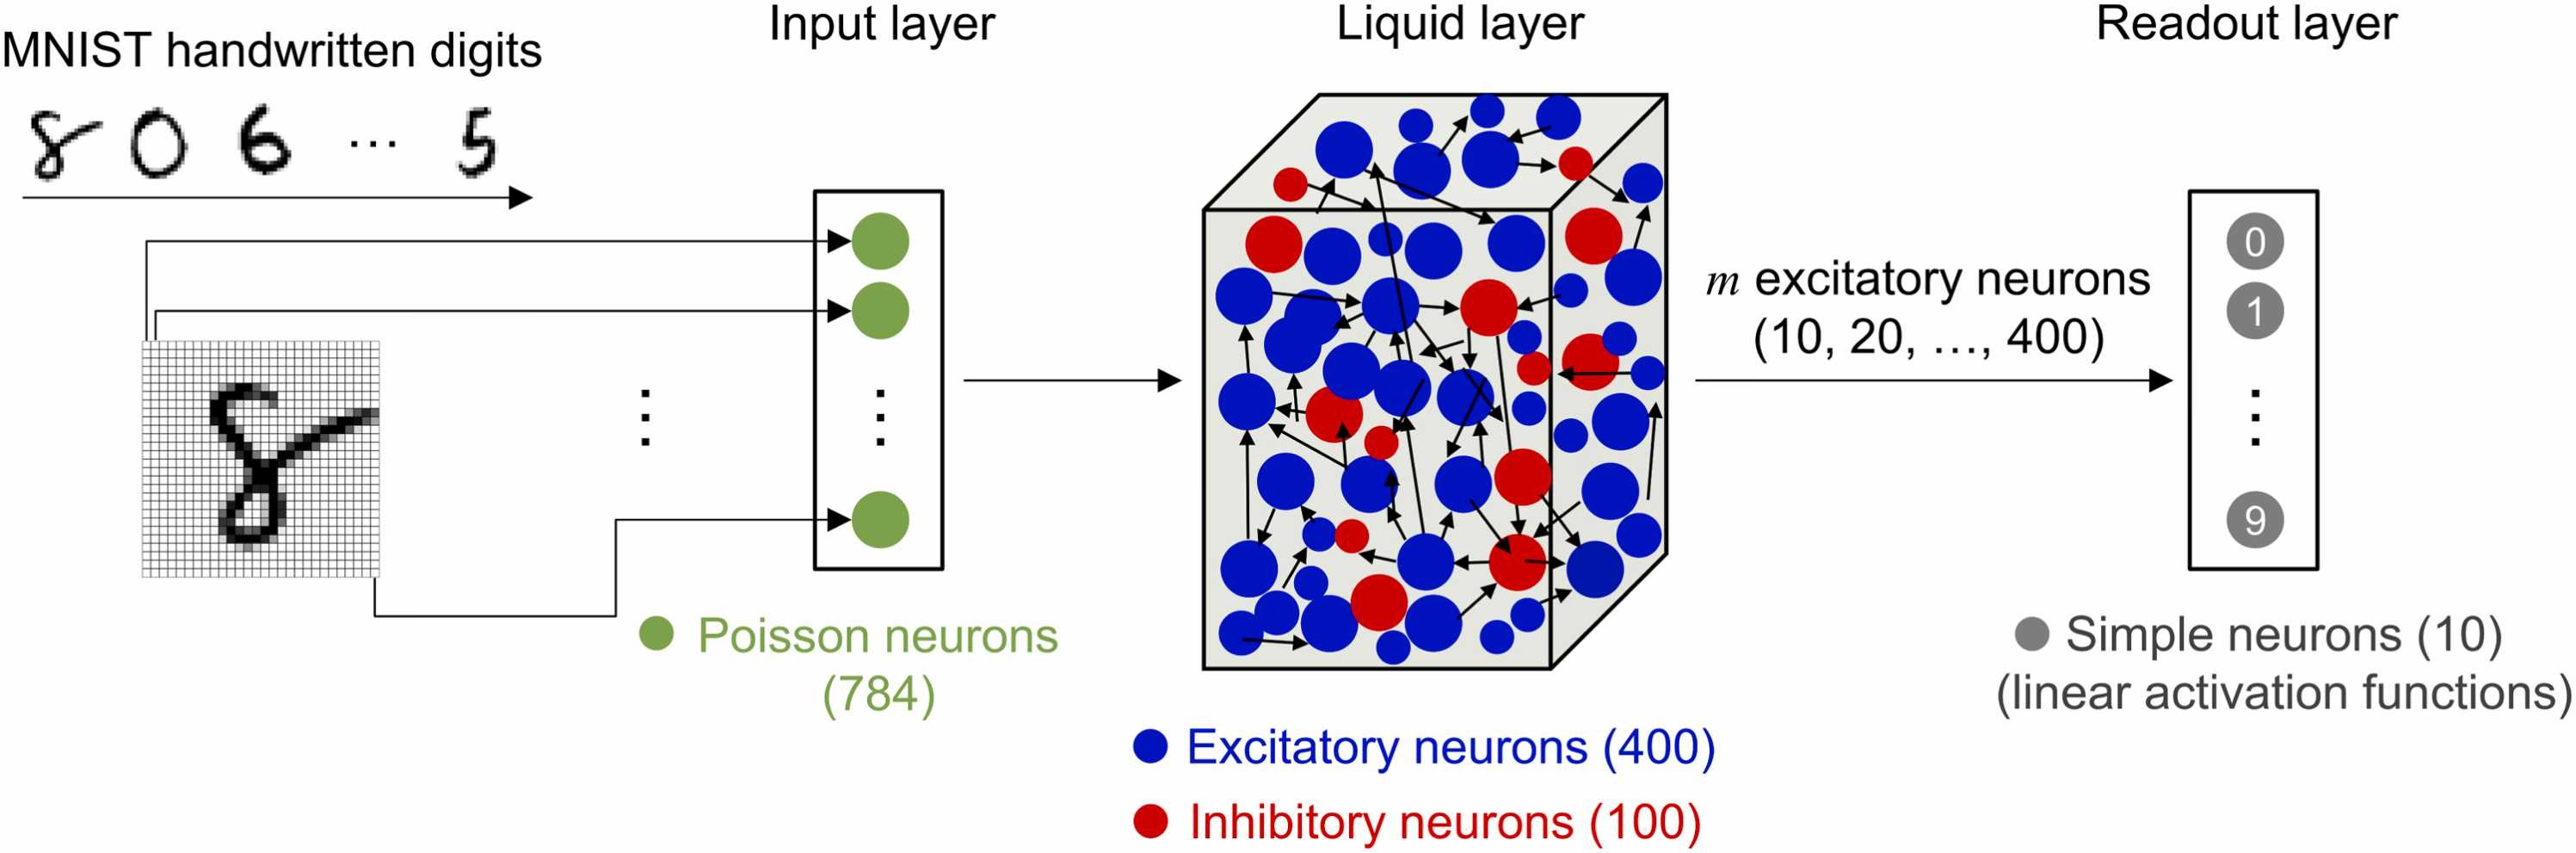
\includegraphics[width=1\linewidth]{figures/lsm_diag.png}
    \caption{Liquid State Machine diagram. \cite{WOO2024129334}}
    \label{fig:enter-label}
\end{figure}

Additionally, physical reservoir computing (PRC) extends these concepts by implementing reservoirs in physical substrates rather than simulating them digitally. This allows exploitation of inherent physical dynamics in materials and systems for computation. As done in one of the papers I worked on implementing: \cite{Mandal2022}.


\subsection{Training Methodology}

The training procedure for reservoir computing is remarkably straightforward compared to traditional neural networks:

\begin{itemize}
    \item Feed input signals into the reservoir and collect the resulting reservoir states
    \item Train a linear readout function (through ridge regression) to map reservoir states to desired outputs
    \item Apply the trained readout to new reservoir states during inference
\end{itemize}
    

The mathematical formulation for this training is typically:
\[
W_{\text{out}} = YG^T\left(GG^T + \lambda I\right)^{-1}
\]
% \[
% \begin{aligned}
% \text{where:} \quad & W_{\text{out}} \text{ is the output weight matrix,} \\
% & Y \text{ is the target output matrix,} \\
% & G \text{ is the matrix of reservoir states,} \\
% & \lambda \text{ is the regularization parameter,} \\
% & I \text{ is the identity matrix.}
% \end{aligned}
% \]
Where $W_{out}$ represents the output weights, $Y$ contains the target outputs, $G$ contains the reservoir states, $\lambda$ is a regularisation parameter, and $I$ is the identity matrix.

\subsection{Advantages and Limitations}

Reservoir computing offers several distinct advantages:
\begin{itemize}
    \item Training involves only linear regression, avoiding complex and computationally intensive backpropagation.
    \item The same reservoir can be used for multiple tasks by training different readout functions.
    \item The fixed nature of the reservoir enables implementation in physical systems.
\end{itemize}


However, there are important limitations as mentioned by \cite{article_catch_22s_rc}: 
\begin{itemize}
    \item The random initialisation provides little control over specific functionalities.
    \item The memory capacity of the reservoir is constrained by its size.
    \item Performance can vary significantly based on the specific task and how well it matches the reservoir's dynamics. \cite{article_RC_intro}
    \item The system in many testing is very much dependent on hyperparameters, and the type of non linear system you select for a particular task.
\end{itemize}



\section{Literature Review}

As seen in this exploratory article \cite{article_RC_intro}, we see how to set up an RC experiment with a given nonlinear system, and highlight the advantage that only the output layer needs training.  

\cite{article_catch_22s_rc} explores limitations of standard RC models in what they call the “Catch-22s”.  They study the problem of basin prediction in multistable systems: determining from an initial condition which attractor the system will approach.  They find that a classic echo state network requires a very long \textit{warm-up} (nearly the full transient trajectory) to correctly predict the basin.  In contrast, a variant called next-generation RC (NGRC) that encodes the exact nonlinear equations can predict basins with almost no warm-up.  However, NGRC’s performance is extremely sensitive: even tiny errors in the presumed nonlinearities make its predictions fail.  In summary, this work shows that standard RC works well for some tasks but struggles with complex basin structure unless aided by precise system knowledge.

\cite{Arun2024} propose using a discrete nonlinear map as the reservoir.  Specifically, they use the logistic map and a finite trigonometric series to create \textit{virtual nodes} of a reservoir.  They demonstrate that this simple reservoir can accurately predict several benchmark tasks: the Lorenz, R\"ossler, and Hindmarsh–Rose systems (temporal tasks) and even a seventh-order polynomial (non-temporal).  Remarkably, their logistic-map reservoir works well even when noisy inputs are present.  The authors report low prediction error (RMSE), indicating the logistic map can serve as an effective high-dimensional reservoir.  Their approach “removes the necessity of continuous dynamical systems for constructing the reservoir” and suggests a general method for time-series prediction using simple discrete maps.

\cite{Mandal2022} examine a physical example of a minimal reservoir.  They use a single driven pendulum (a simple nonlinear mechanical oscillator) as the reservoir.  Through both simulation and a proof-of-principle experiment, they show that this one-dimensional system can perform standard RC tasks.  The key is to exploit the pendulum’s rich transient dynamics: they feed an input signal as a driving torque, record the pendulum’s angle and angular velocity over time, and train the output on those signals.  Surprisingly, even this "minimal one-node reservoir" achieved good accuracy on temporal (predicting time series) and non-temporal tasks.  This work indicates that even a very low-dimensional physical system can have considerable “learning potential” when used as a reservoir.

Finally, \cite{Itoh2020} focus on reconstructing bifurcation diagrams from data.  They generate time-series data from an electronic circuit (a discrete-time chaotic system) across different parameter values, including dynamical and observational noise.  Using an Extreme Learning Machine (ELM) – a single-hidden-layer feedforward network with random weights – they train a predictor to map time-series inputs to future values.  By sweeping the input parameter and using the ELM predictions, they successfully reconstruct the system’s bifurcation diagram.  Importantly, their method proved robust: the reconstructed Lyapunov exponents matched those from the true system, showing accurate attractor structure recovery even in noisy conditions.  This demonstrates that machine learning (via ELM) can infer global bifurcation behaviour from limited time-series data.

\section{Implementation and Results}

This section contains some of the experiments that I implemented and tested about various reservoir computing systems, inspired by the literature above.  

\subsection{Pendulum Reservoir}\label{pendulum_res}
Firstly, I simulated a driven pendulum as a reservoir, following the approach of \cite{Mandal2022}.  The pendulum dynamics are given by the standard nonlinear equation (including damping and an external driving torque). 

As the input signal, we inject a time-varying driving force as the reservoir state, and record the pendulum’s angle and angular velocity.  These two scalar values at each time were concatenated into a state vector.  Over a sequence of inputs, the pendulum produces a rich time series in its transient motion.  

The dynamics of the driven damped pendulum are governed by the following system of differential equations:
\begin{equation}
\begin{aligned}
\frac{dx}{dt} &= v, \\
\frac{dv}{dt} &= -\frac{g}{l} \sin(x) - k v + f \, \text{sign}(\sin(\omega t)),
\end{aligned}
\label{eq:pendulum}
\end{equation}
where
\begin{itemize}
    \item $x(t)$ is the angular displacement,
    \item $v(t)$ is the angular velocity,
    \item $g$ is the gravitational acceleration,
    \item $l$ is the length of the pendulum,
    \item $k$ is the damping coefficient,
    \item $f$ is the amplitude of the external periodic forcing,
    \item $\omega$ is the forcing frequency,
    \item and $\text{sign}(\cdot)$ is the signum function.
\end{itemize}


We collected these state histories and trained a linear output layer to predict a target time series (for example, reconstructing the input signal after a delay).  We found that the pendulum reservoir could learn the task to a useful degree of accuracy, similar to the findings of the paper. Figure~\ref{fig:pendulum-1} shows the results of a predicted graph just based on $x_{t-1}$. I believe I could get better results, and that it is not perfect due to RC being highly dependent on the hyperparameters set. But this experiment shows that a simple single oscillator can function as an effective reservoir for learning time-dependent tasks.

\begin{figure}[H]
    \centering
    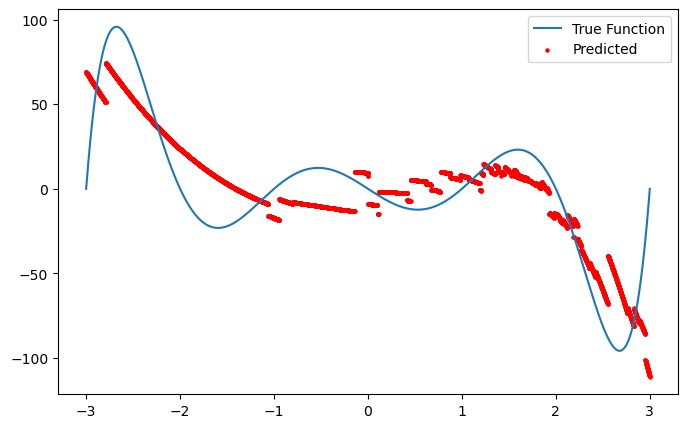
\includegraphics[width=0.75\linewidth]{figures/pendulum_result_0.png}
    \caption{Results of the single pendulum reservoir experiment.}
    \label{fig:pendulum-1}
\end{figure}

The Lorenz system is a classic example of a chaotic dynamical system, described by the following set of ordinary differential equations:
\begin{equation}
\begin{aligned}
\frac{dx}{dt} &= \sigma (y - x), \\
\frac{dy}{dt} &= x (\rho - z) - y, \\
\frac{dz}{dt} &= x y - \beta z,
\end{aligned}
\label{eq:lorenz}
\end{equation}
where $\sigma$, $\rho$, and $\beta$ are positive parameters controlling the dynamics. In this standard Lorenz system, the parameters are set to
\[
\sigma = 10, \quad \rho = 28, \quad \beta = \frac{8}{3}.
\]
These equations are solved numerically with an initial condition $\mathbf{x}(0) = (x_0, y_0, z_0)$. In this project, time series data is generated by integrating the Lorenz equations with initial state $(1, 1, 1)$ over a time span of $t \in [0, 100]$ using 10,000 points.

For training the reservoir computing model, the $x$-component of the Lorenz system is used as the input sequence, and the reservoir is trained to predict the full state vector $(x, y, z)$ at the next time step.

\begin{figure}[H]
    \centering
    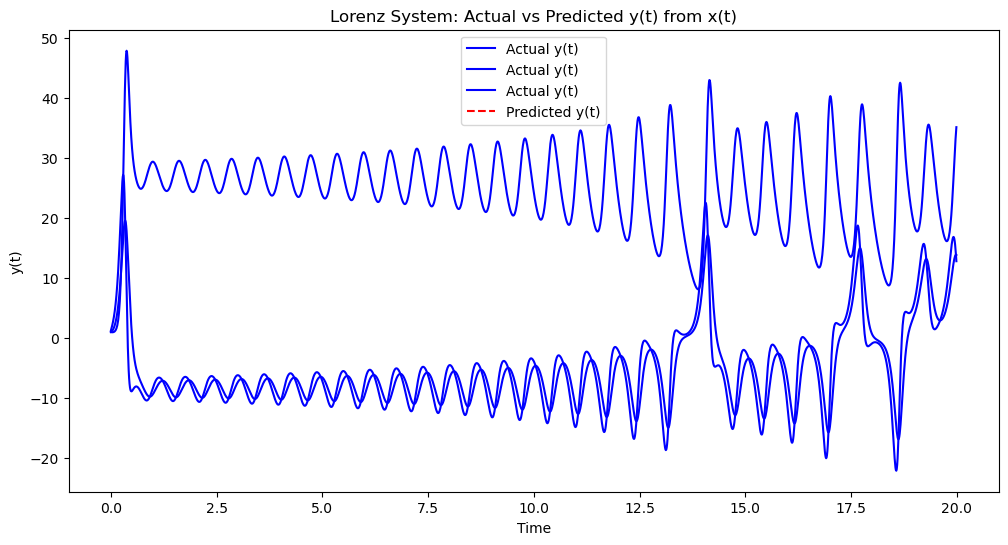
\includegraphics[width=1\linewidth]{figures/lorentz_pendulum_1.png}
    \caption{Actual vs Predicted for the Lorentz system using Pendulum reservoir}
    \label{fig:lorentz_1}
\end{figure}

\begin{figure}[H]
    \centering
    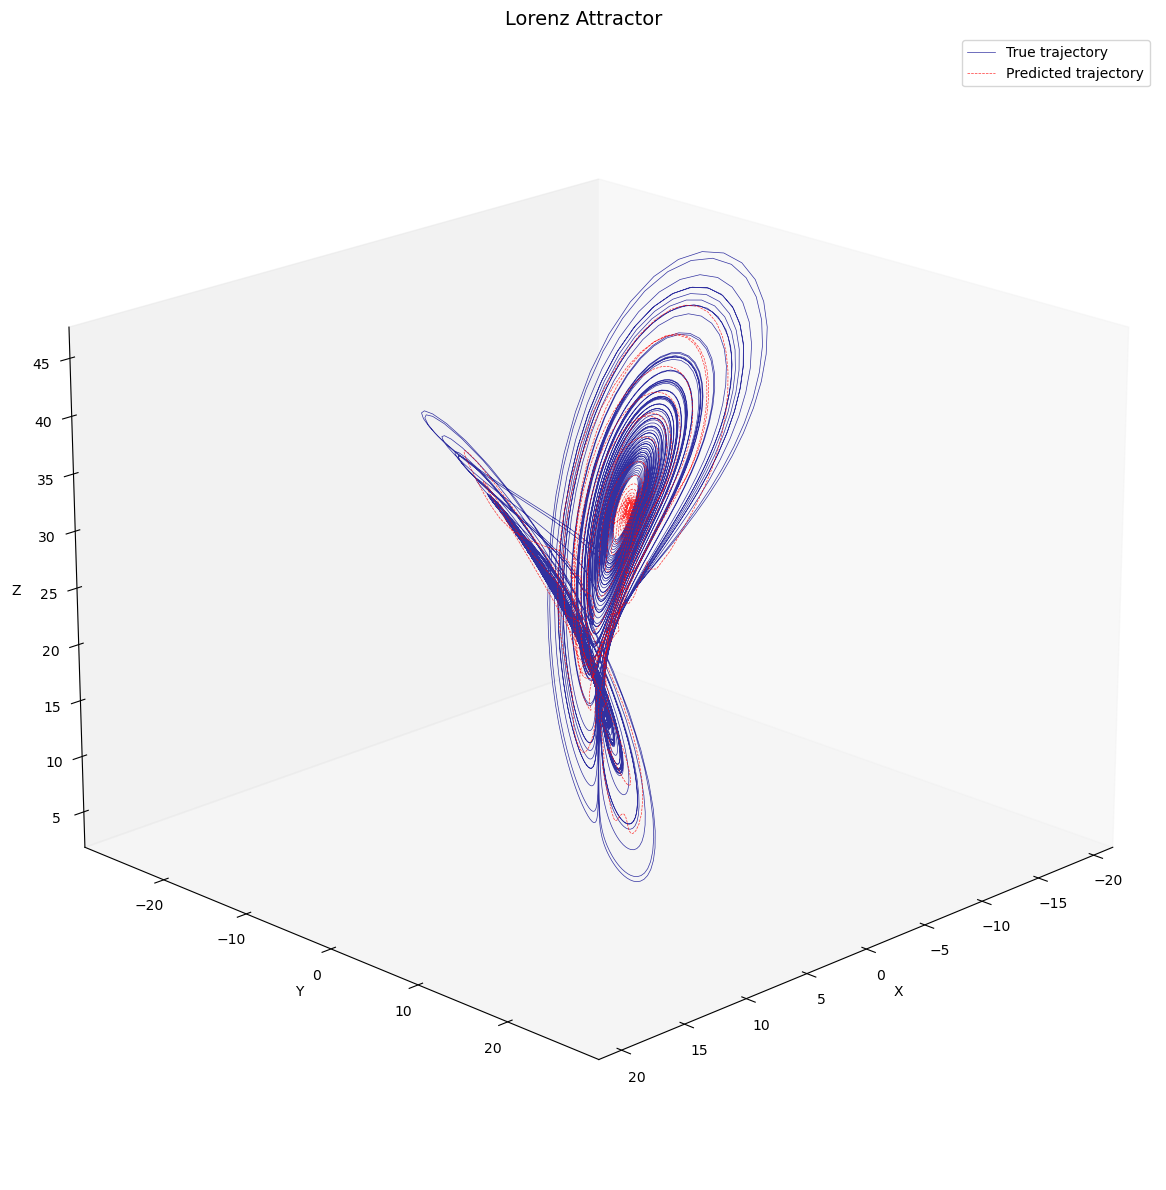
\includegraphics[width=1\linewidth]{figures/lorentz_pendulum_2.png}
    \caption{3D render of actual vs Predicted timestep}
    \label{fig:lorentz_2}
\end{figure}

% Code for the pendulum reservoir experiments: \ref{code_lorenz_pendulum}


\subsection{Logistic Map Reservoir}
A reservoir was also constructed using the logistic map, as described by \cite{Arun2024}.  The logistic map $x_{n+1} = r x_n (1-x_n)$ is iterated to generate a sequence.  To create a high-dimensional reservoir, the technique of \emph{virtual nodes} is used: for each new input, the logistic map is updated several times (with fixed parameter $r$) and its values sampled at intermediate steps, possibly combined with a simple trigonometric expansion as in the paper. Here, a 7th-degree polynomial was set as a micro-benchmark, which is used in many other reservoir computing papers as well.

These sampled values form the reservoir state vector.  The output layer is then trained on this state to predict a time-series target (for example, forecasting the future state of a chaotic system).  The results (as seen in Figure~\ref{fig:logistic_map}) show that the logistic-map reservoir could indeed predict a chaotic time series with relatively low error.  Noise perturbations in the input had only a minor effect, consistent with the robustness reported by the paper as well. This validates that even a discrete map can act as an effective reservoir model.

\begin{figure}[H]
    \centering
    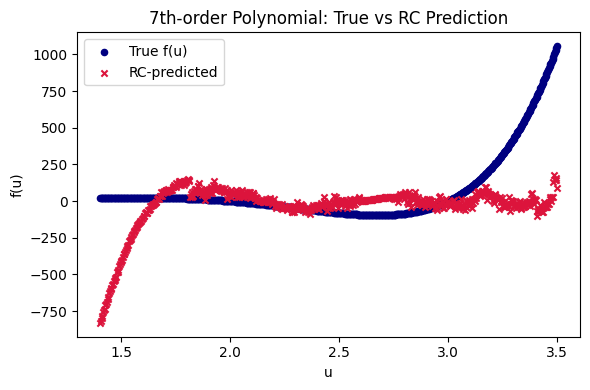
\includegraphics[width=0.75\linewidth]{figures/logistic_7th_degree.png}
    \caption{Results using Logistic Map to then try to map to a target polynomial.}
    \label{fig:logistic_map}
\end{figure}

Now, as implemented for \hyperref[pendulum_res]{Pendulum Reservoir}, a similar problem is tried but using this logisitic map's system. Doing that the following results are obtained: \ref{fig:logistic_map_lorenz} \ref{fig:logistic_map_lorenz_diag}.

\textbf{Test RMSE (x,y,z): [3.76673884 2.93538559 8.36222649]}

\begin{figure}[H]
    \centering
    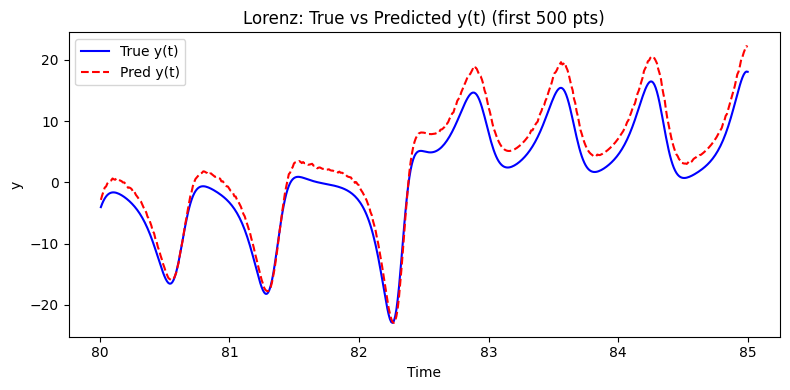
\includegraphics[width=1\linewidth]{figures/lorentz_logistic_pred_true.png}
    \caption{Results for the Lorenz attractor using Logistic Map}
    \label{fig:logistic_map_lorenz}
\end{figure}

\begin{figure}[H]
    \centering
    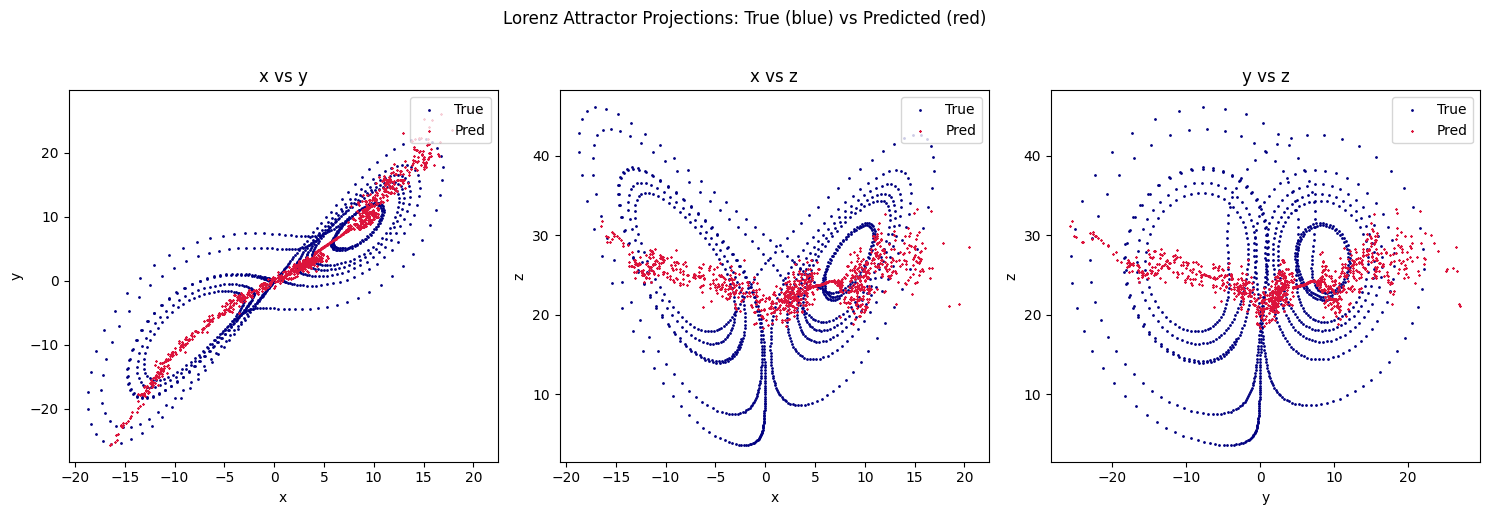
\includegraphics[width=1\linewidth]{figures/lorenz_logistic_pred_diagram.png}
    \caption{Results for the Lorenz attractor using Logistic Map, evolution of different axes over time.}
    \label{fig:logistic_map_lorenz_diag}
\end{figure}

% Code for the logistic map reservoir for polynomial: \ref{code_logistic_polynomial}

% Code for the logistic map reservoir for Lorenz system: \ref{code_logistic_lorenz}


\subsection{Bifurcation Reconstruction via PCA and ELM}\label{BD_recon_section}
Reconstruction of bifurcation diagram of a nonlinear system using reservoir outputs, inspired by \cite{Itoh2020} is tried.  The procedure is as follows: for a range of a system parameter $\mu$, run the simulations of the system and feed its time-series data through the reservoir (logistic reservoirs).  

The reservoir state responses are collected for each parameter value. Principal Component Analysis (PCA) is applied to reduce dimensionality to the reservoir states, extracting the leading modes as features. Then an Extreme Learning Machine (ELM) regressor is trained to map these PCA features (plus the parameter $\mu$) to a predicted system output (the next state or an observable).  By sweeping $\mu$ and using the trained ELM predictions, the goal is to trace the transitions of attractor values versus $\mu$.  

Figure~\ref{fig:bifurcation} shows results for the reconstructed diagram.  It is found that reconstruction is incomplete: some bifurcation branches are missing, distorted, or just weird.  The ELM managed to learn local trends of the data to some extent, but it does not capture the full global structure. This was in contrast to the paper that achieved robust reconstructions.  The imperfect result may be due to limited training data, noise, an insufficient reservoir or wrong implementation. The authors have not shared their implementation, just a vague description of hyperparameters.  The replicated implementation could also have a high chance of being incorrect/incomplete to an extent. 

\begin{figure}[H]
    \centering
    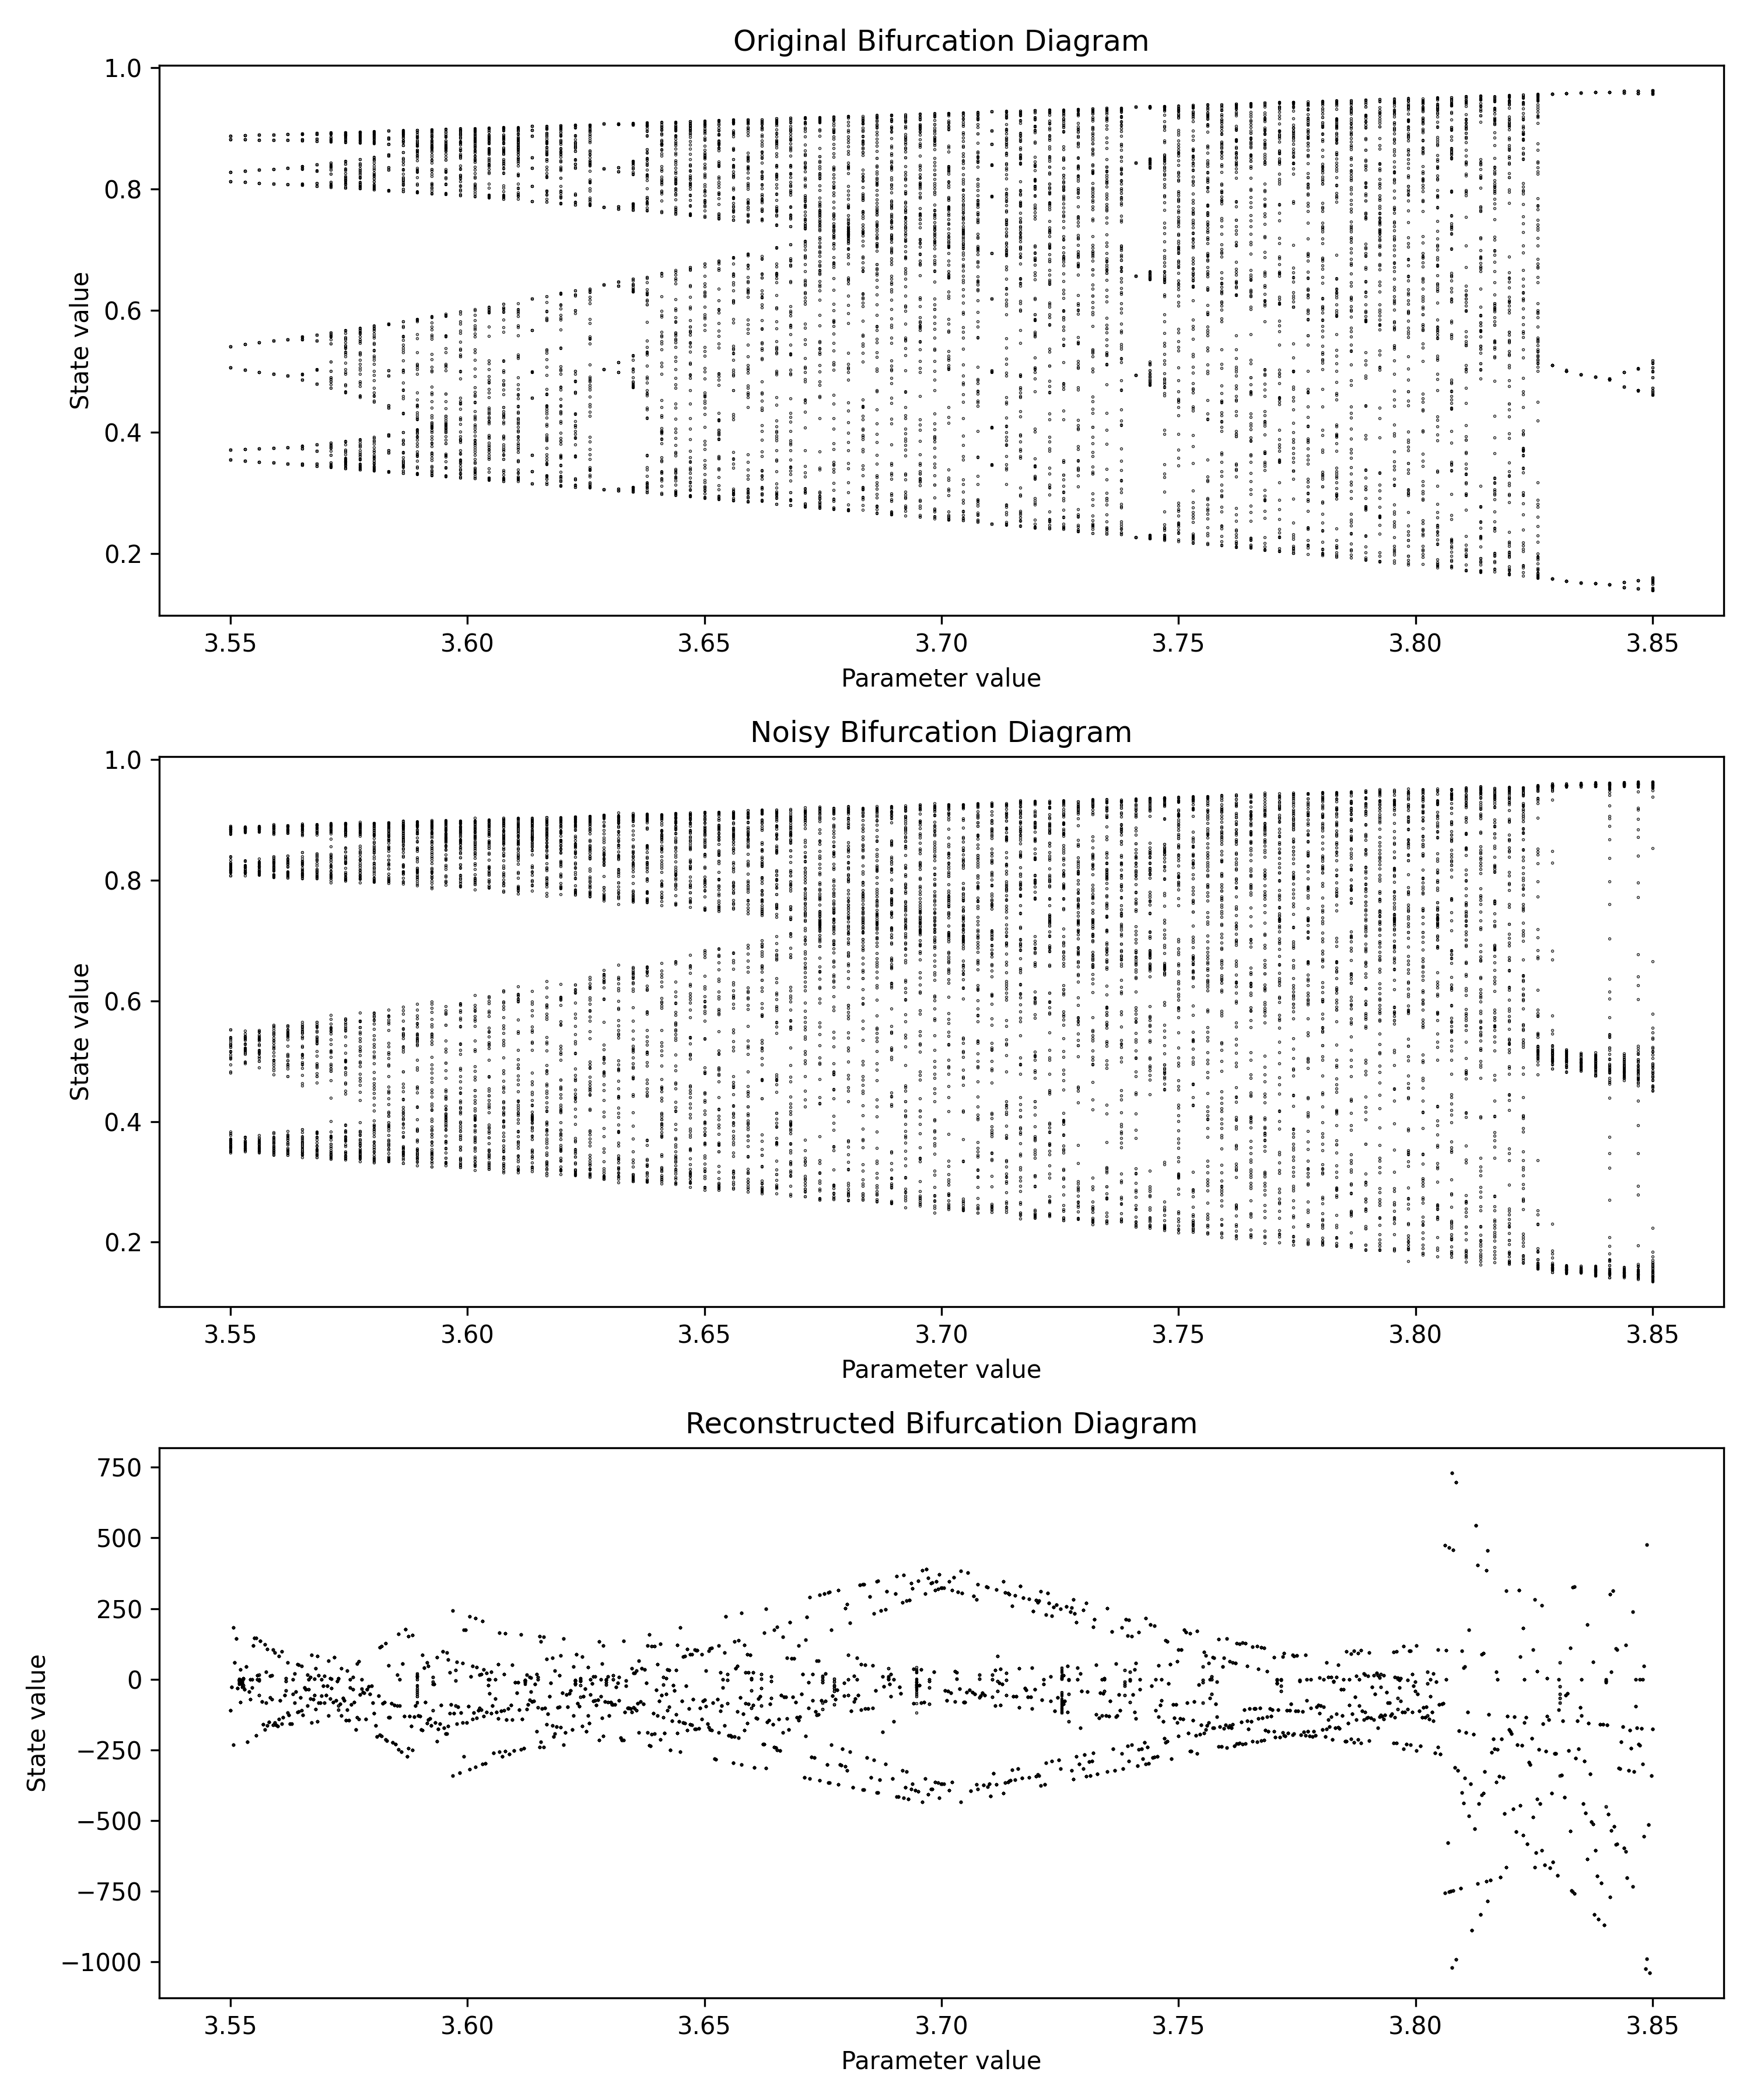
\includegraphics[width=1\linewidth]{figures/bd_reconstruction_elm.png}
    \caption{The first attempt at reconstruction of a system's bifurcation diagram using reservoir PCA + ELM}
    \label{fig:bifurcation}
\end{figure}

After some more fine-tuning and fixing a lot of issues, these are some results that seem much better than the original ones.

\begin{figure}[H]
    \centering
    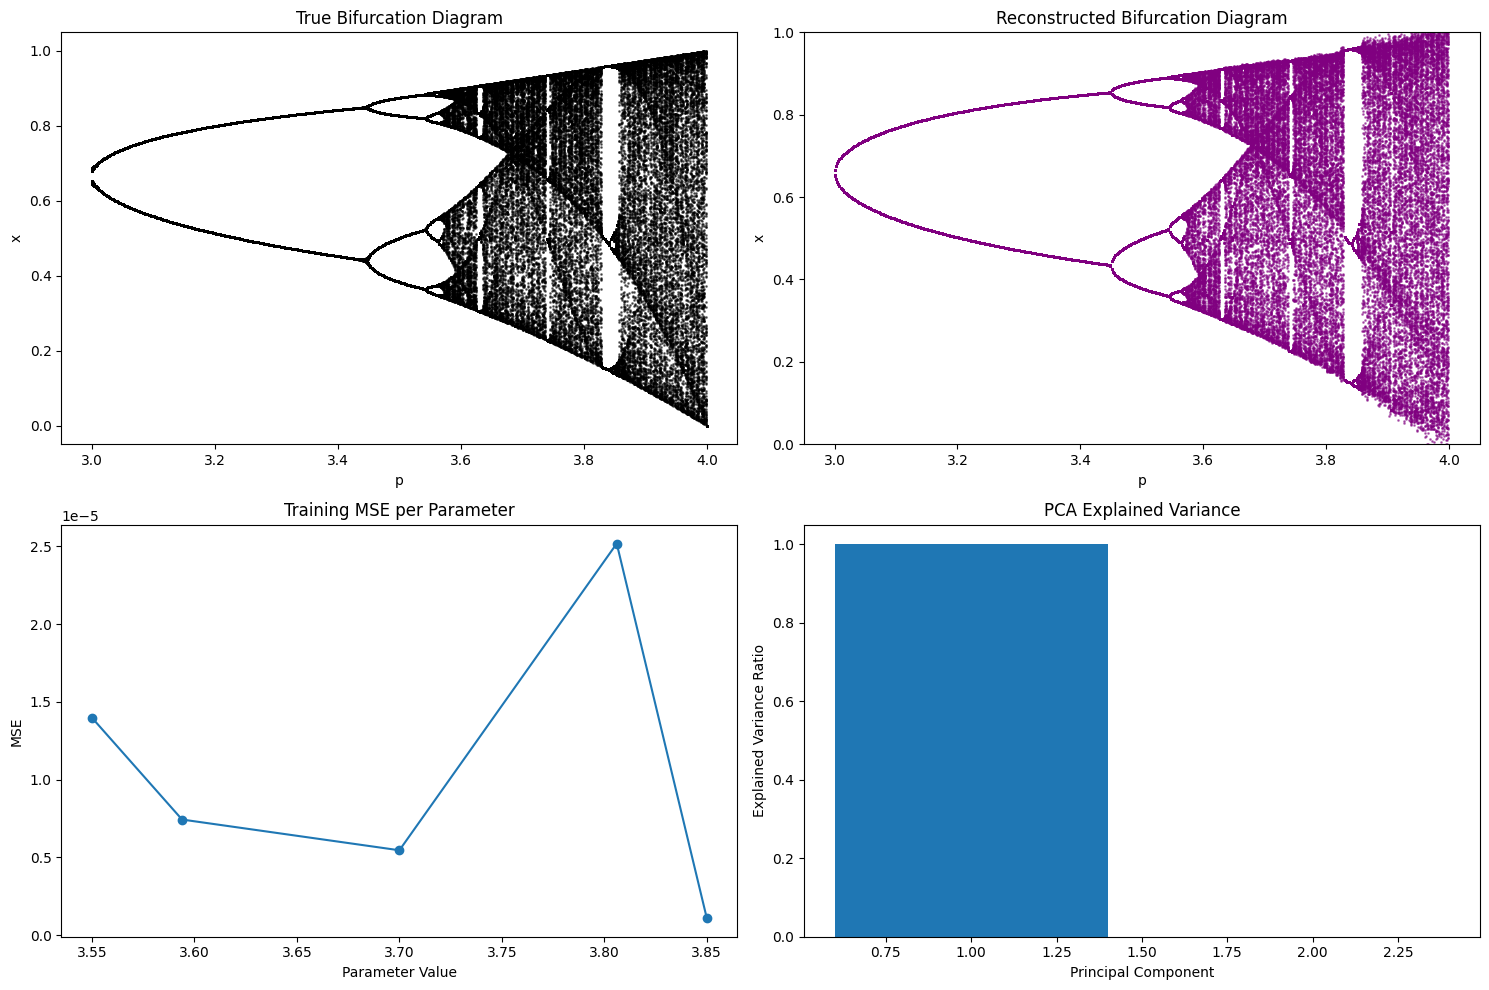
\includegraphics[width=1\linewidth]{figures/bd_1_results.png}
    \caption{Training MSE: 1.06e-05. Code for this implementation:}
    \label{fig:bd_1}
\end{figure}

\begin{figure}[H]
    \centering
    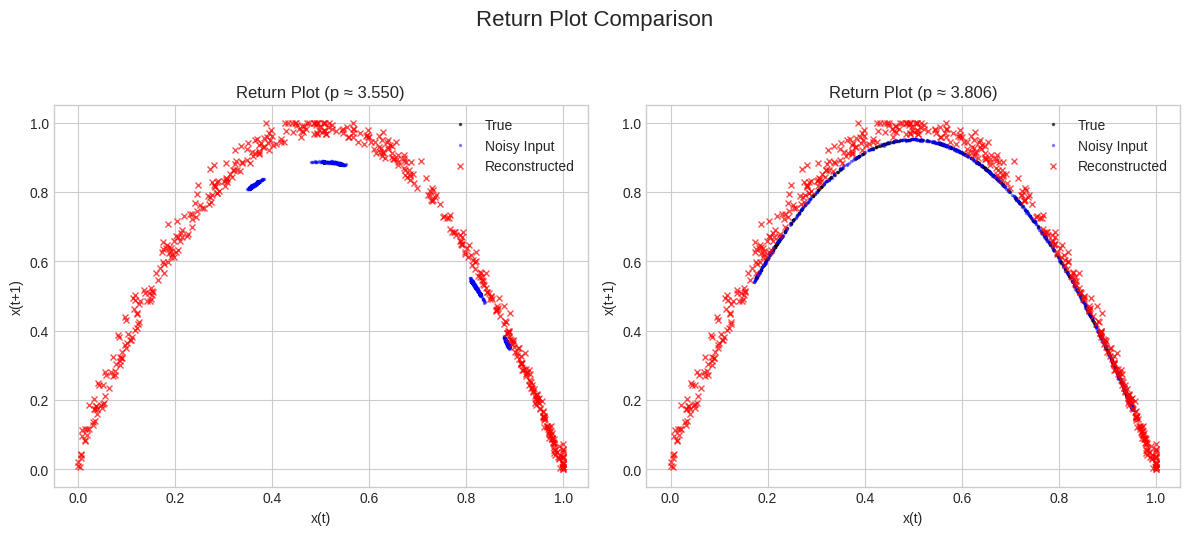
\includegraphics[width=1\linewidth]{figures/bd_return_plot_2.png}
    \caption{One of the visualisations in the paper was reconstructing the return plot, i.e., $x_{(t+1)}$ vs $x_t$}
    \label{fig:bd_2}
\end{figure}

\begin{figure}[H]
    \centering
    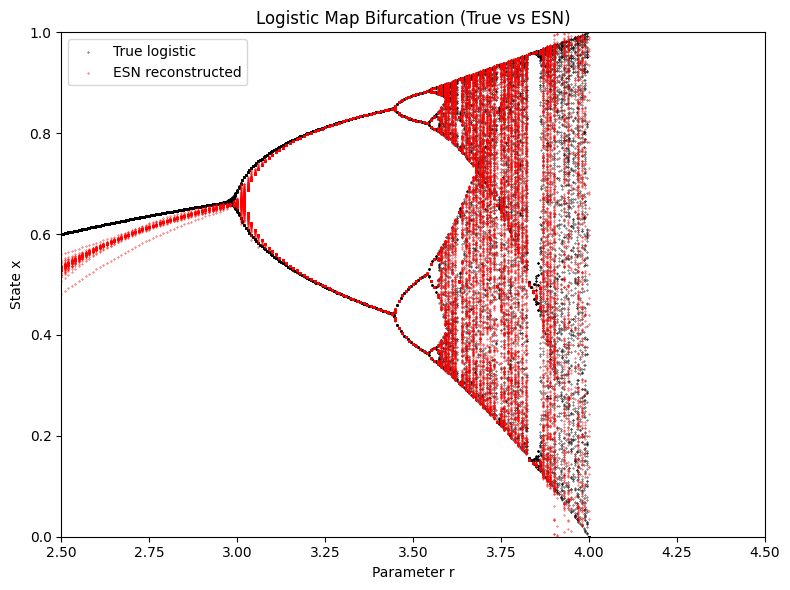
\includegraphics[width=0.8\linewidth]{figures/bf_3_results_overlapped.png}
    \caption{Plot of the overlapping true and predicted bifurcation diagrams. The issue remains that the predictions outside the trained parameter space are not very accurate.}
    \label{fig:bd_3}
\end{figure}

\begin{figure}[H]
    \centering
    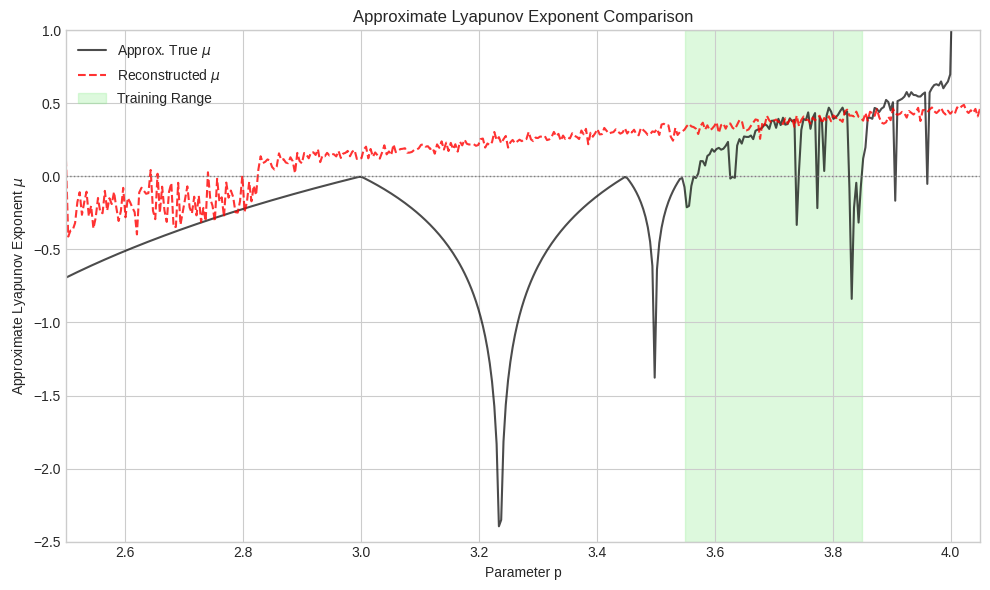
\includegraphics[width=1\linewidth]{figures/lyapanov_bd_rd.png}
    \caption{Using the reservoir model to estimate approximate Lyapunov exponents for different parameter values. The system as only trained on the highlighted green region of the graphs, it is estimating the exponent for other parameter values.}
    \label{fig:lypanov_bd_rc}
\end{figure}


\begin{figure}[H]
    \centering
    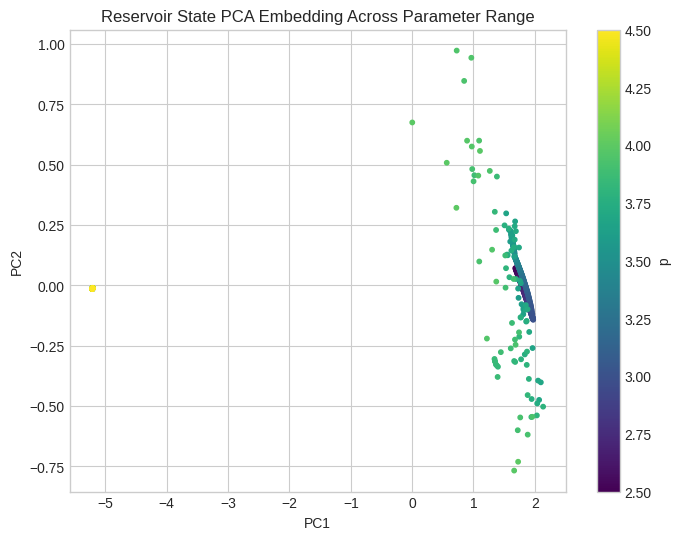
\includegraphics[width=0.8\linewidth]{figures/bd_elm_pca_analysis.png}
    \caption{Analysis of the PCA components for different parameters yields an interesting correlation. Almost like a straight line being fit through the values with slope of -1. }
    \label{fig:bd_4}
\end{figure}

\begin{figure}[H]
    \centering
    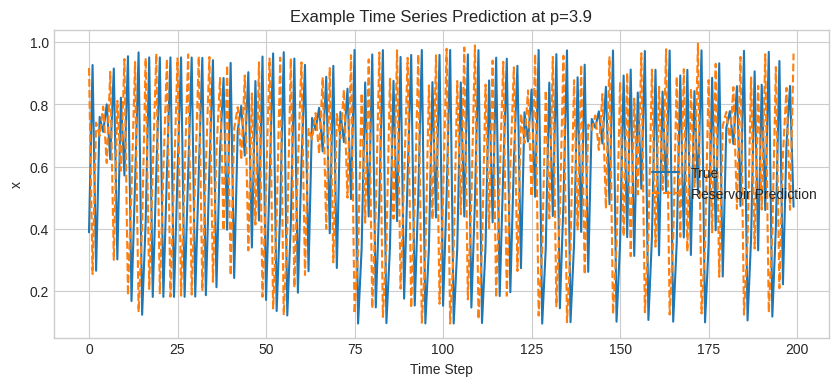
\includegraphics[width=01.0\linewidth]{figures/bd_5_prediction_for_specific_value.png}
    \caption{Predicting the evolution using the trained ELM for a random parameter value.}
    \label{fig:bd_5}
\end{figure}

% \subsection{Using Recurrent Networks}

% - with above RC, was not getting perfect results, either due to hyperparameter search or whatever reason it may be
% - lets try some recurrent network to learn the space and see how well does it understand and can make bifurcation diag
% - used LSTMs
% - actually works and we get decent results

\subsection{Using Recurrent Networks (LSTM) for Reconstruction}

Initial attempts using a single Reservoir Computing (RC) model (like Echo State Network - ESN) trained on combined time-series data from different parameter values ($p$) failed to accurately reconstruct the bifurcation diagram, often yielding noise-like output \ref{fig:bd_2}. This occurred because the fixed reservoir and single readout could not effectively disentangle the parameter-dependent behaviour required for reconstruction.


\begin{figure}[H]
    \centering
    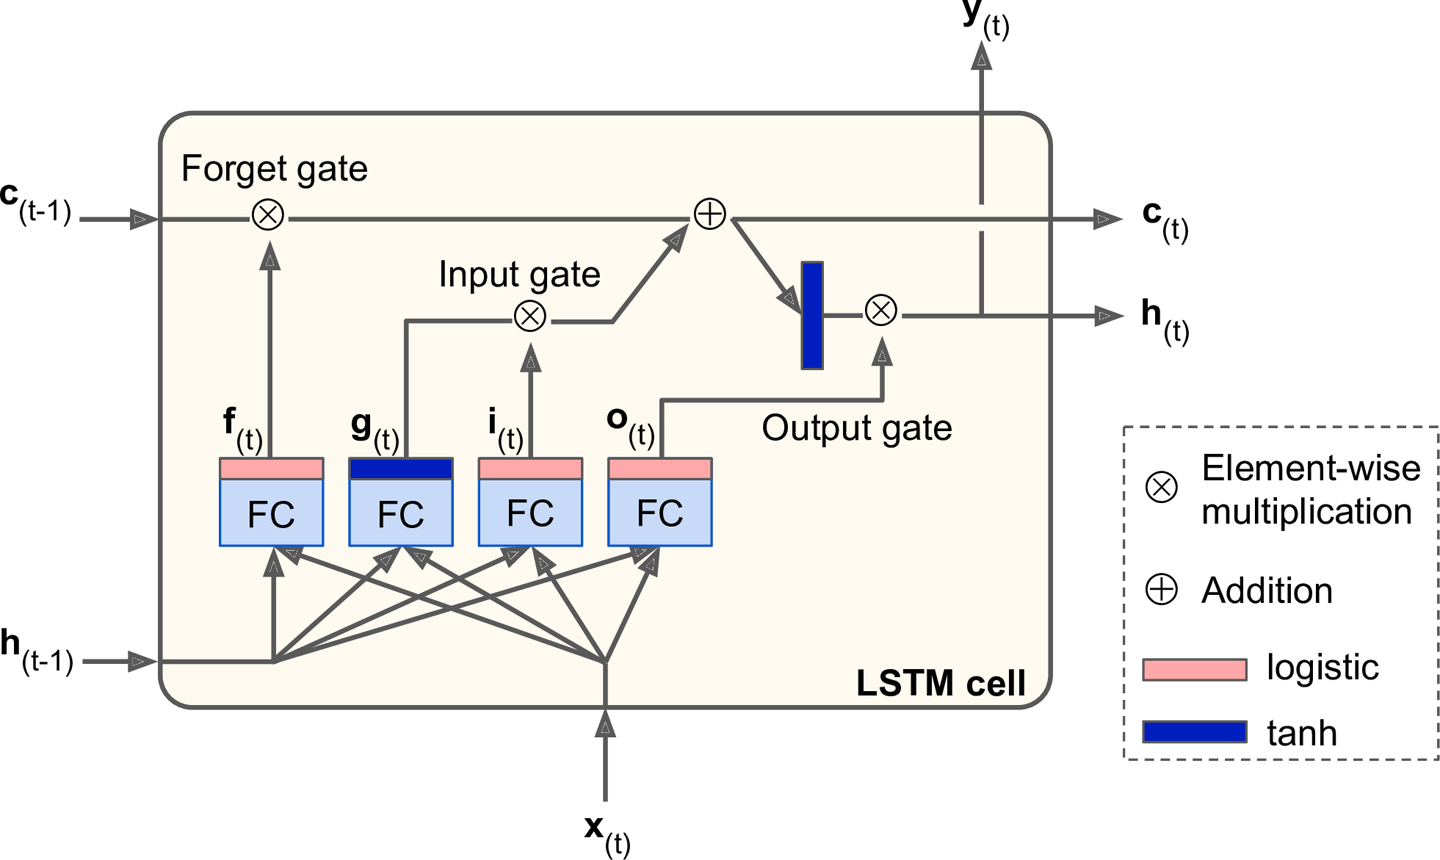
\includegraphics[width=1\linewidth]{figures/LSTM_arch.png}
    \caption{Long Short-Term Memory (LSTM) architecture}
    \label{fig:lstm_arch}
\end{figure}

An alternative approach using a Long Short-Term Memory (LSTM) network, a type of Recurrent Neural Network (RNN), proved more successful. The key differences enabling this approach to work better are:

\begin{enumerate}
    \item \textbf{Parameter as Explicit Input:} Unlike the previous ESN implementation \ref{BD_recon_section}, the LSTM model is explicitly designed to take both the current state $x_t$ and the bifurcation parameter $p$ as inputs to predict the next state $x_{t+1}$. The learned mapping is:
    \begin{equation}
        \hat{x}_{t+1} = g_{\text{LSTM}}(x_t, p; \theta)
        \label{eq:lstm_map}
    \end{equation}
    where $\theta$ represents all trainable weights (including recurrent connections) of the LSTM.

    \item \textbf{Learning Conditional Dynamics:} The single LSTM model is trained using data aggregated from all available training parameters $\{p_n\}$. By receiving $p$ as input, the network learns the conditional dynamics $x_{t+1} | (x_t, p)$ across the sampled parameter range, rather than averaging the dynamics as in the initial ESN attempt.

    \item \textbf{End-to-End Training:} All weights $\theta$ within the LSTM are adjusted during training (via backpropagation). This allows the network's internal recurrent dynamics to adapt specifically for modelling how the system's behaviour changes with $p$, offering potentially more representational power than the fixed, random reservoir of a standard ESN/ELM.

    \item \textbf{Reconstruction via Iteration:} The trained LSTM $g_{\text{LSTM}}$ is iterated autonomously for any desired parameter $p^*$ to generate attractor points:
    \begin{equation}
        \hat{x}_{t+1} = g_{\text{LSTM}}(\hat{x}_t, p^*; \theta)
    \end{equation}
\end{enumerate}


In short, the LSTM's ability to directly incorporate the parameter $p$ as input and learn the parameter-conditioned dynamics through full network training seems to be a good explanation of its superior performance compared to the initial single-ESN implementation, which lacked this explicit parameter handling. This LSTM approach remains distinct from the ELM + PCA method \ref{BD_recon_section}, which identifies parameter space through PCA on the output weights of separately trained predictors.

\begin{figure}[!htbp]
    % \centering
    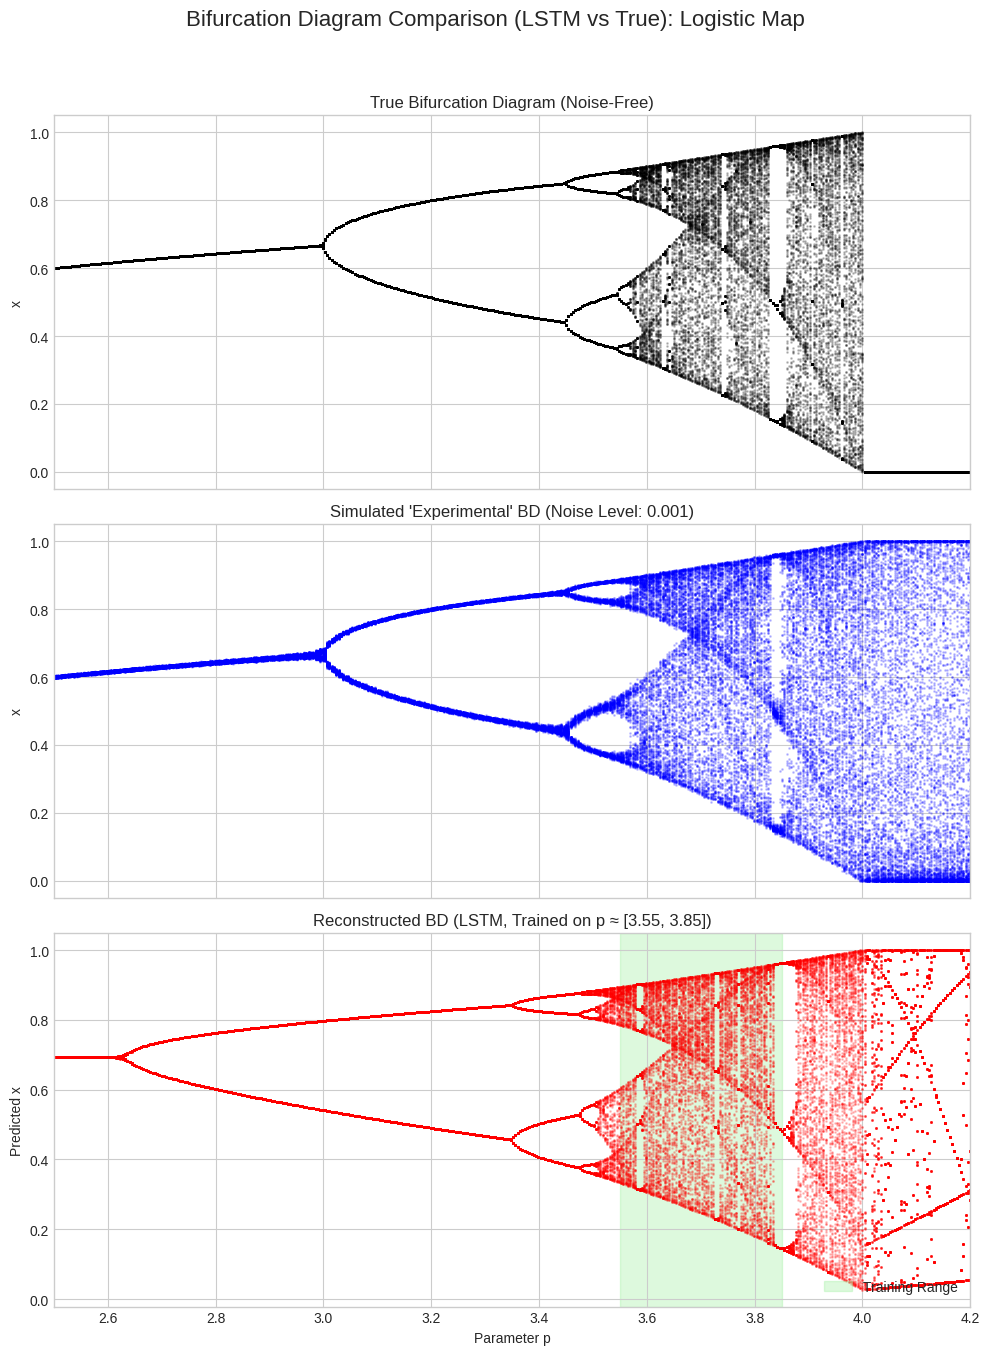
\includegraphics[width=1.0\linewidth]{figures/lstm_bd_1.png}
    \caption{Comparison shown with reconstruction of the Bifurcation diagram using LSTM.  In the reconstructed BD graph, the highlighted green region is the only region for which the model was trained. The rest is reconstructing how the model thinks the system would evolve for different parameter values.}
    \label{fig:lstm_bd_1}
\end{figure}\FloatBarrier

% rest of the caption
%  

\begin{figure}[!htbp]
    \centering
    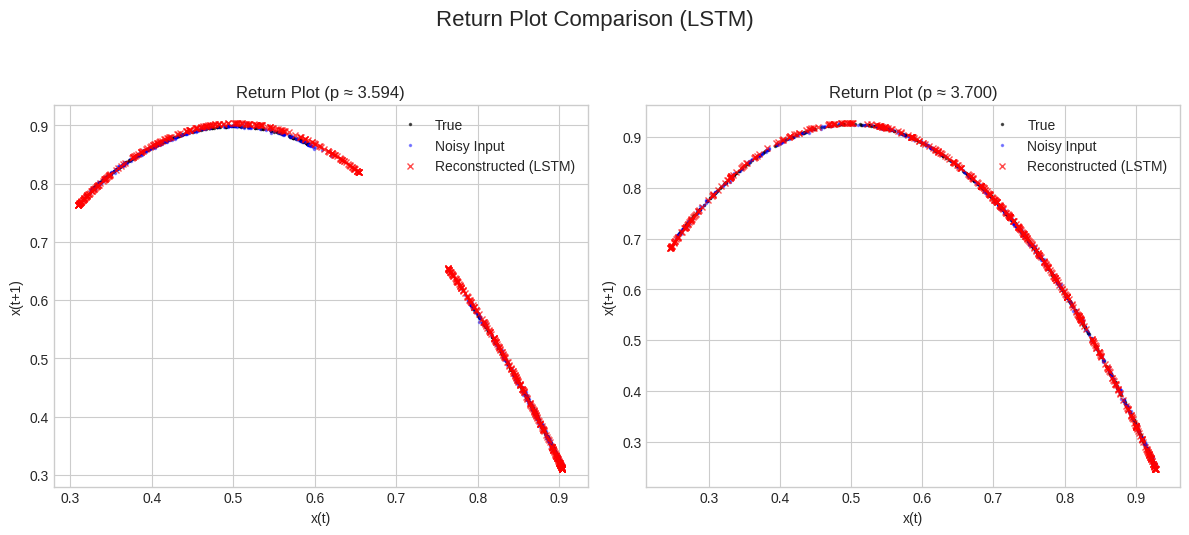
\includegraphics[width=1\linewidth]{figures/lstm_bd_2.png}
    \caption{Reconstruction of evolution of $x_{(t+1)}$ vs $x_t$ for different parameter values.}
    \label{fig:lstm_bd_2}
\end{figure}
\FloatBarrier

\begin{figure}[!htbp]
    \centering
    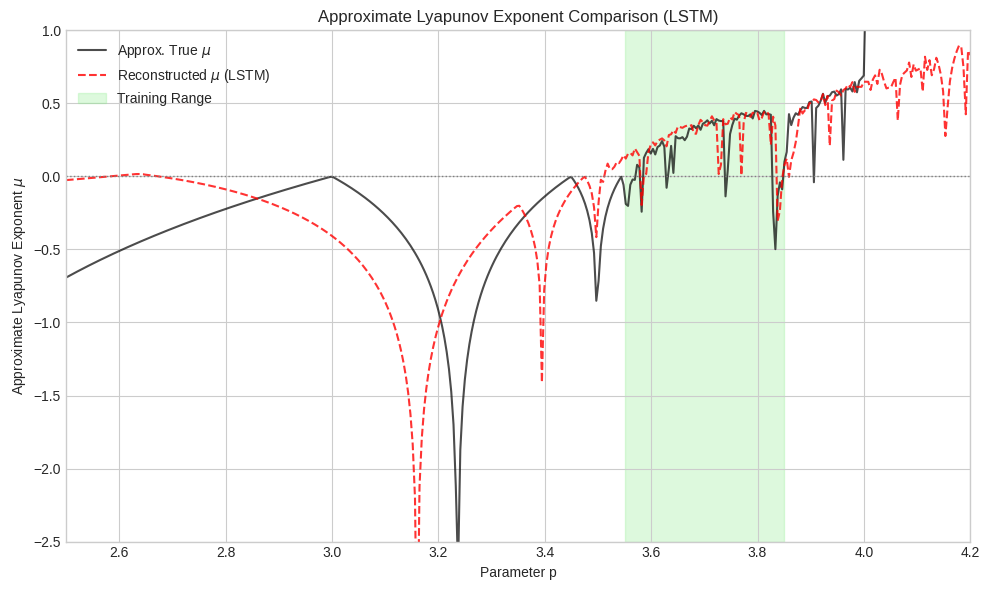
\includegraphics[width=1\linewidth]{figures/lstm_bd_3.png}
    \caption{Using the model to estimate the approximate Lyapunov exponent for different parameter values. Again, like others, the green region highlights the training data limit.}
    \label{fig:enter-label}
\end{figure}
\FloatBarrier


The primary difference in terms of usability was that the LSTM model took around \textbf{46 seconds} to train while the regression ELM took \textbf{less than a second}. 

This performance gain is especially because of training only the output layer is where reservoir computing performs extremely well. But due to compute being so much cheaper and efficient in most modern problems, sequential models - be it as rudimentary as RNNs, or newer approaches like Transformers or State Space Models (Mamba) \cite{gu2024mambalineartimesequencemodeling} could be a better fit for such problems. 

\section{Conclusion}

This project explored the application of reservoir computing (RC), one of the tasks that involves utilising an Extreme Learning Machine (ELM) combined with Principal Component Analysis (PCA), to reconstruct bifurcation diagrams from simulated noisy time-series data. The goal was to emulate data analysis from physical systems like electronic circuits, using the logistic map as a case study. While the approach successfully reproduced the broad features of the period-doubling route to chaos present in the logistic map, it fundamentally failed to capture fine structures within the chaotic regions or to accurately extrapolate beyond the parameter range used during training. These limitations underscore the challenges posed by noise and the sensitivity to RC hyperparameter configurations.

Beyond the specific results, this investigation provided valuable insights into the practical implementation and characteristics of RC. I learned about the core principles of RC, including its massive efficiency while training when compared to traditional recurrent networks, and its potential for modelling nonlinear systems directly from time-series data. The project highlighted scenarios where RC's ability to process temporal information with minimal training overhead could be advantageous, particularly in contexts involving physical systems where obtaining clean data or precise system models is difficult. 

However, the difficulties encountered in accurately reconstructing complex dynamics and extrapolating outside the trained parameter space emphasise the trade-offs inherent in the RC approach and the need for tuning and potentially hybrid methods for more demanding prediction tasks. 

In hindsight, I feel Recurrent networks are more suited for all of these tasks, especially as now computing is not a major limiting factor in most research work. 

\section{Future Work}

Future efforts could focus on improving the fidelity and robustness of the bifurcation diagram reconstruction. Optimisation of RC hyperparameters (reservoir size, spectral radius, leaking rate, input scaling, regularisation) as well as using techniques like Bayesian optimisation could be essential to potentially overcome the observed limitations in capturing fine structures and improving extrapolation. 

Applying the methodology to a wider array of dynamical systems would further test its generality. This includes investigating higher-dimensional maps, continuous-time systems (requiring considerations for numerical integration or time-delay embedding), systems exhibiting different bifurcation types (Hopf, saddle-node), and coupled systems to assess scalability. 

Comparing the performance with alternative RC architectures, such as deep reservoir networks or different readout mechanisms beyond ELM, could identify more effective configurations for this specific task. 

Finally, validating the simulation results by applying the reconstruction technique to time-series data obtained from actual physical hardware, such as electronic circuits, pendulums, or other systems, which kind of motivated this study, would provide insights into its real-world applicability and limitations.


%%%%%%%%%%%%%%%%%%%%%%%%%%%%%%%%%%%%%%%%%%%%%%%%%%%%%%%%%%%%%%%%%%%%%%
%% Bibliography
%%%%%%%%%%%%%%%%%%%%%%%%%%%%%%%%%%%%%%%%%%%%%%%%%%%%%%%%%%%%%%%%%%%%%%

% \section*{References}
% \bibliographystyle{plainnat}
% \bibliography{references}

\clearpage
\addcontentsline{toc}{section}{References}
\renewcommand{\bibsection}{\section*{References}}
\bibliographystyle{plainnat}
\bibliography{references}






%%%%%%%%%%%%%%%%%%%%%%%%%%%%%%%%%%%%%%%%%%%%%%%%%%%%%%%%%%%%%%%%%%%%%%
%% Acknowledgements
%%%%%%%%%%%%%%%%%%%%%%%%%%%%%%%%%%%%%%%%%%%%%%%%%%%%%%%%%%%%%%%%%%%%%%
\addcontentsline{toc}{section}{Acknowledgement}
\section*{Acknowledgement}

I would like to thank \textbf{\href{https://www.bits-pilani.ac.in/goa/gaurav-dar/}{Prof. Gaurav Dar}} for his guidance, insights and motivating me throughout this project. 


\end{document}